\documentclass[tikz,border=10pt]{standalone}
\usepackage{pgfplots}
\usepgfplotslibrary{groupplots}
\pgfplotsset{compat=1.18}

\begin{document}
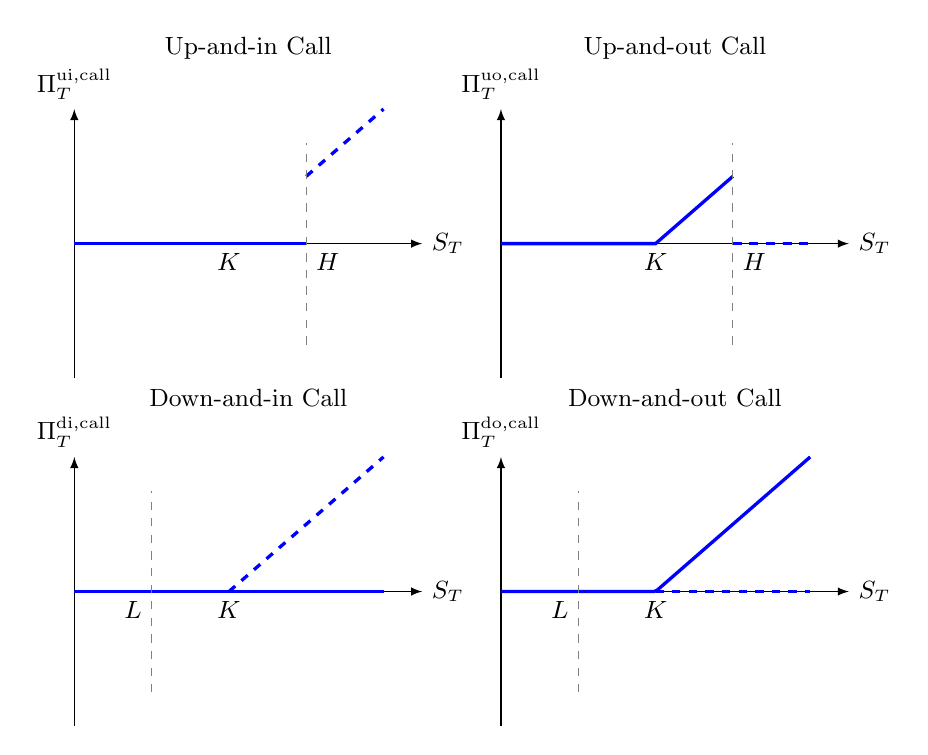
\begin{tikzpicture}[font=\small]

  \pgfmathsetmacro{\K}{2}
  \pgfmathsetmacro{\L}{1}
  \pgfmathsetmacro{\H}{3}

  \begin{groupplot}[
      group style={
          group size=2 by 2,
          horizontal sep=1cm,
          vertical sep=1cm,
        },
      width=6cm, height=5cm,
      axis lines=middle,
      axis line style={-latex},
      xmin=0, xmax=4.5,
      ymin=-2, ymax=2,
      xtick=\empty, ytick=\empty,
      domain=0:4,
      samples=100,
      every axis plot/.style={blue, very thick, no marks},
      xlabel={$S_T$},
      xlabel style={at={(axis description cs:1,0.5)}, anchor=west},
      title style={
          at={(axis description cs:0.5,1)},
          yshift=0.3cm,
          anchor=south,
        },
      clip=false,
    ]

    % up-and-in call
    \nextgroupplot[
      ylabel={$\Pi_T^\mathrm{ui,call}$},
      ylabel style={at={(axis description cs:0,1)}, anchor=south},
      title={Up-and-in Call},
    ]
    \addplot[domain=0:\H] {0};
    \addplot[domain=\H:4, dashed] {max(x-\K,0)};
    \draw (axis cs:\K,0) node[below] {$K$};
    \draw[dashed, gray] (axis cs:\H, -1.5) -- (axis cs:\H, 1.5);
    \draw (axis cs:\H,0) node[anchor=north west] {$H$};

    % up-and-out call
    \nextgroupplot[
      ylabel={$\Pi_T^\mathrm{uo,call}$},
      ylabel style={at={(axis description cs:0,1)}, anchor=south},
      title={Up-and-out Call},
    ]
    \addplot[domain=0:\H] {max(x-\K,0)};
    \addplot[domain=\H:4, dashed] {0};
    \draw (axis cs:\K,0) node[below] {$K$};
    \draw[dashed, gray] (axis cs:\H, -1.5) -- (axis cs:\H, 1.5);
    \draw (axis cs:\H,0) node[anchor=north west] {$H$};

    % down-and-in call
    \nextgroupplot[
      ylabel={$\Pi_T^\mathrm{di,call}$},
      ylabel style={at={(axis description cs:0,1)}, anchor=south},
      title={Down-and-in Call},
    ]
    \addplot[domain=0:4] {0};
    \addplot[domain=\K:4, dashed] {max(x-\K,0)};
    \draw (axis cs:\K,0) node[below] {$K$};
    \draw[dashed, gray] (axis cs:\L, -1.5) -- (axis cs:\L, 1.5);
    \draw (axis cs:\L,0) node[anchor=north east] {$L$};

    % down-and-out call
    \nextgroupplot[
      ylabel={$\Pi_T^\mathrm{do,call}$},
      ylabel style={at={(axis description cs:0,1)}, anchor=south},
      title={Down-and-out Call},
    ]
    \addplot {max(x-\K,0)};
    \addplot[domain=\K:4, dashed] {0};
    \draw (axis cs:\K,0) node[below] {$K$};
    \draw[dashed, gray] (axis cs:\L, -1.5) -- (axis cs:\L, 1.5);
    \draw (axis cs:\L,0) node[anchor=north east] {$L$};

  \end{groupplot}
\end{tikzpicture}
\end{document}